
\subsubsection{2007: Heckmann et al.}
\label{sec:heckmann}

A different approach is implemented by~\citet{heckmann_gumogeneral_2005}.
Divided into four main groups (emotional state, personality, characteristics and
physiological state), the authors present the \acf{gumo}, an ontology model to 
characterize users capabilities within adaptive environments. A significant 
user aspect that is taken into account in this work is the stress. In the 
adaptive interfaces domain it is needed to pay special attention to the 
consequences of each adaptation. But the stress is not only determined  by this 
process. It is also derived from several user experiences, as the current 
context state (e.g. traffic, noise, surrounding people, and so 
forth~\citep{babisch_noise_stress_2002}). Figure~\ref{fig:heckmann_model} illustrates
the model presented by~\citeauthor{heckmann_gumogeneral_2005}.

% \InsertFig{heckmann_model}{fig:heckmann_model}{Several user model property
% dimensions~\citep{heckmann_gumogeneral_2005}}{}{0.70}{}

\begin{figure}
\centering
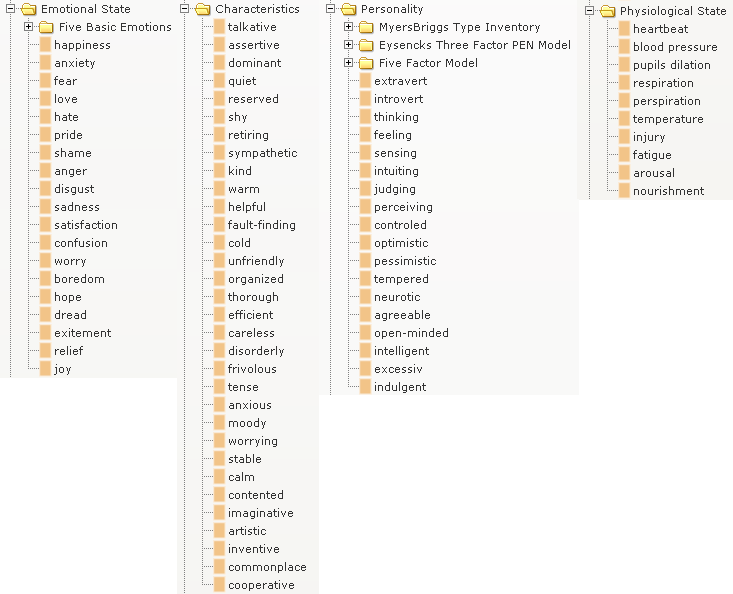
\includegraphics[width=0.60\textwidth]{heckmann_model.png}
\caption{Several user model property
dimensions~\citep{heckmann_gumogeneral_2005}.}
\label{fig:heckmann_model}
\end{figure}

% ----------------------------------------------------------------------